\label{chap:dataset_preprocessing}

\section{Introduction to the Multi-Modal Cohort}
Personalized metabolic modeling requires high-dimensional, time-synchronized physiological and nutritional data collected under free-living, real-world human conditions. In this thesis, we utilize the comprehensive \textbf{CGMacros} study cohort \cite{mendes2024cgmacros}. The dataset monitors 45 human participants over multi-week free-living protocols, capturing complete postprandial glycemic excursions alongside lifestyle, dietary, biometric, and metagenomic streams.

\section{Clinical Cohort Demographics and Metabolic Stratification}
The 45 human participants encompass three clinically distinct metabolic strata:
\begin{itemize}
    \item \textbf{Healthy Controls ($n=12$):} Normoglycemic individuals exhibiting normal fasting plasma glucose ($\text{FPG} < 100\text{ mg/dL}$) and glycated hemoglobin ($\text{HbA1c} < 5.7\%$).
    \item \textbf{Pre-Diabetes ($n=16$):} Individuals with impaired fasting glucose or impaired glucose tolerance ($\text{HbA1c} \in [5.7\%, 6.4\%]$).
    \item \textbf{Type 2 Diabetes ($n=17$):} Diagnosed diabetic individuals exhibiting elevated glycemia ($\text{HbA1c} \ge 6.5\%$ or receiving anti-diabetic pharmacotherapy).
\end{itemize}

Figure \ref{fig:hba1c_distribution} illustrates the distribution of baseline clinical glycated hemoglobin (HbA1c \%) across the three clinical sub-cohorts, confirming the wide metabolic spectrum represented in the digital twin training and validation population.

\begin{figure}[!h]
\centering
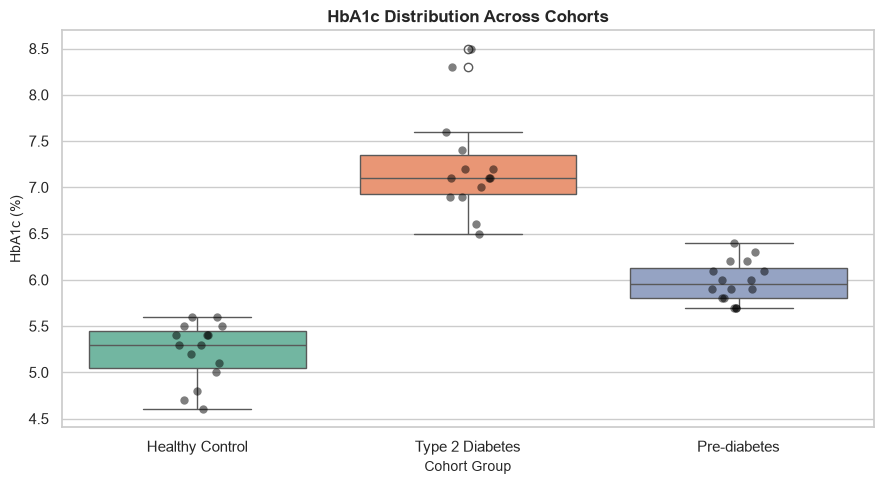
\includegraphics[width=0.75\columnwidth]{images/hbaic_distribution_across_cohorts.png}
\caption{Clinical distribution of baseline HbA1c (\%) across Healthy, Pre-diabetes, and Type 2 Diabetes participants in the CGMacros cohort.}
\label{fig:hba1c_distribution}
\end{figure}

\section{The Five Heterogeneous Data Modalities}
The CGMacros cohort unites five heterogeneous physiological and behavioral modalities:

\begin{enumerate}
    \item \textbf{Continuous Dual CGM Telemetry:} Participants simultaneously wore two distinct continuous glucose sensors on opposing upper arms:
    \begin{itemize}
        \item Abbott FreeStyle Libre (Flash glucose monitoring with 1-minute interpolation).
        \item Dexcom G6 (Real-time enzymatic glucose monitoring recorded at 1-minute intervals).
    \end{itemize}
    This dual-sensor configuration provides interstitial fluid glucose concentrations in milligrams per deciliter ($\text{mg/dL}$).
    
    \item \textbf{Wearable Physical Activity and Biometrics:} Continuous telemetry captured via wrist-worn commercial fitness trackers (Fitbit), recording:
    \begin{itemize}
        \item Photoplethysmography (PPG) Heart Rate (BPM).
        \item Metabolic Equivalent of Task (METs), recording minute-by-minute physical exertion.
        \item Estimated caloric energy expenditure ($\text{kcal/min}$).
    \end{itemize}
    
    \item \textbf{Dietary Macronutrient Logs:} Granular real-time dietary logging of all consumed meals and beverages. Each meal record includes the precise start timestamp, total energy (kcal), carbohydrates (g), dietary fiber (g), free sugars (g), total fat (g), and protein (g).
    
    \item \textbf{Diagnostic Laboratory Blood Panel:} Baseline clinical fasting venous blood samples, providing:
    \begin{itemize}
        \item Fasting Plasma Glucose (FPG, $\text{mg/dL}$).
        \item Fasting Plasma Insulin ($\mu\text{IU/mL}$).
        \item Homeostatic Model Assessment of Insulin Resistance (HOMA-IR $= \frac{\text{FPG} \times \text{Insulin}}{405}$).
        \item Glycated Hemoglobin (HbA1c \%).
        \item Complete Lipid Panel: Total Cholesterol, High-Density Lipoprotein (HDL), Low-Density Lipoprotein (LDL), and Triglycerides ($\text{mg/dL}$).
    \end{itemize}
    
    \item \textbf{Gut Microbiome Metagenomic Profiles:} Stool metagenomic sequencing yielding:
    \begin{itemize}
        \item 22 gut functional health indices (including Short-Chain Fatty Acid / Butyrate Synthesis and Lipopolysaccharide / LPS Biosynthesis).
        \item High-dimensional binary taxonomic presence-absence indicators across 1,979 discrete bacterial species.
    \end{itemize}
\end{enumerate}

Figure \ref{fig:butyrate_distribution} depicts the functional microbial Butyrate Synthesis capacity score stratified across the clinical diagnostic cohorts, highlighting the marked depletion of beneficial SCFA-producing microbial pathways in individuals with Type 2 Diabetes.

\begin{figure}[!h]
\centering
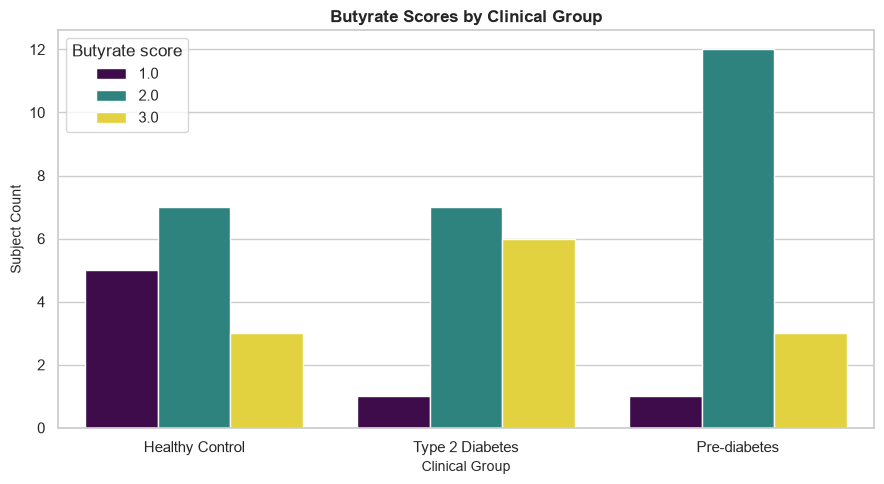
\includegraphics[width=0.75\columnwidth]{images/butyrate_scores_by_clinical_group.png}
\caption{Gut microbiome functional Butyrate Synthesis scores across metabolic groups, demonstrating marked microbial depletion in Type 2 Diabetes.}
\label{fig:butyrate_distribution}
\end{figure}

\section{Dual CGM Sensor Harmonization and Imputation}
Operating commercial CGM sensors in free-living environments introduces challenges of inter-sensor drift, physiological latency (due to glucose transit time between intravascular blood and interstitial tissue), and transient wireless signal dropouts. 

To create a single, robust, continuous physiological telemetry stream, we developed a dual-sensor harmonization pipeline. When both sensors are operating concurrently, the unified glucose signal $G_{\text{unified}}(t)$ is computed via sensor averaging:
\begin{equation}
G_{\text{unified}}(t) = 
\begin{cases}
\frac{G_{\text{Libre}}(t) + G_{\text{Dexcom}}(t)}{2}, & \text{if } G_{\text{Libre}}(t) \text{ and } G_{\text{Dexcom}}(t) \text{ are active} \\
G_{\text{sensor}}(t), & \text{if only a single sensor is active}
\end{cases}
\end{equation}

Figure \ref{fig:dual_sensor_comparison} visualizes the raw telemetry signals from both sensors across an exemplary multi-day monitoring period, demonstrating inter-sensor concordance as well as transient localized drift.

\begin{figure}[!t]
\centering
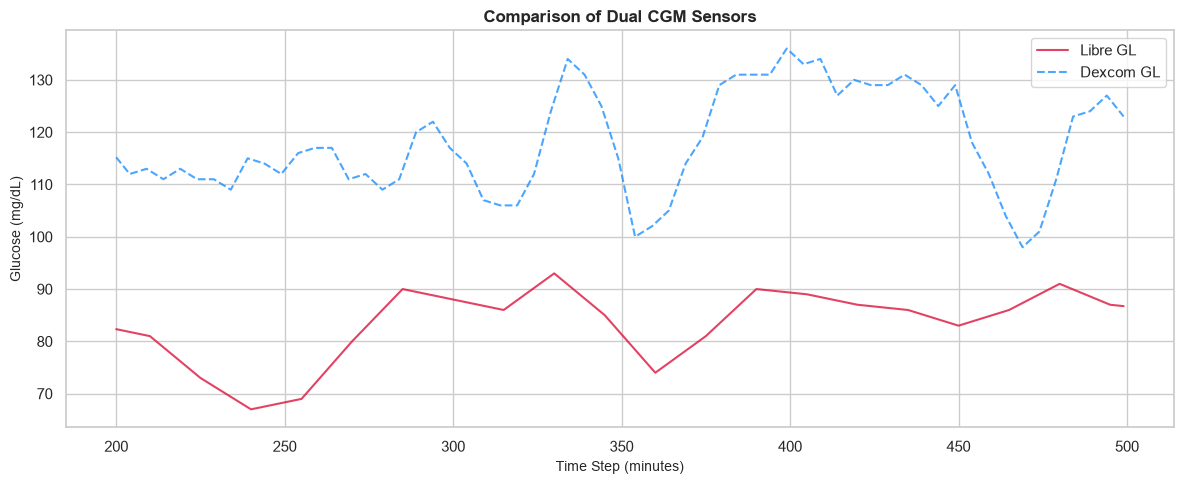
\includegraphics[width=0.9\columnwidth]{images/comparison_of dual_cgm_sensors.png}
\caption{Time-synchronized telemetry comparing simultaneous Abbott FreeStyle Libre and Dexcom G6 glucose streams across representative monitoring days.}
\label{fig:dual_sensor_comparison}
\end{figure}

Transient signal dropouts ($\le 15$ minutes) were imputed using shape-preserving piecewise linear interpolation. Missing heart rate values were imputed via forward and backward filling anchored to the cohort median resting rate (70 BPM). Missing activity records defaulted to baseline resting sedentary METs ($10.0$ on the raw scale, corresponding to $1.0\text{ MET}$). Figure \ref{fig:sanitized_signal} shows the final, sanitized continuous glucose signal resulting from this pipeline.

\begin{figure}[!h]
\centering
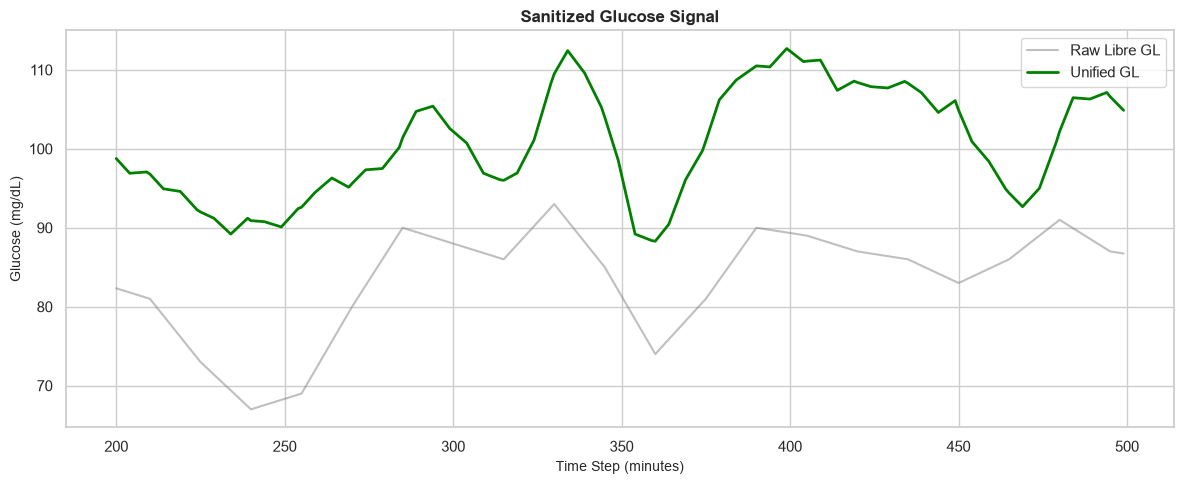
\includegraphics[width=0.9\columnwidth]{images/sanitized_glucose_signal.png}
\caption{Sanitized, unified continuous glucose signal following artifact rejection, sensor harmonization, and dropout interpolation.}
\label{fig:sanitized_signal}
\end{figure}

\section{Macronutrient Scale Correction and Energy Balance}
Exploratory audit of the raw dietary database revealed mixed scale anomalies where participant logging software fluctuated between fractional ($0.0 - 1.0$) and percentage ($1.0 - 100.0$) representations for \texttt{Amount Consumed}. Uncorrected, fractional entries would underestimate consumed macronutrients by two orders of magnitude ($100\times$). 

We implemented an automated normalization filter: all records with \texttt{Amount Consumed} $> 1.0$ were divided by $100.0$. Net ingested grams for carbohydrates, dietary fiber, sugars, fats, and proteins were then computed:
\begin{equation}
    \text{Macronutrient}_{\text{net}}\text{ (g)} = \text{Macronutrient}_{\text{logged}}\text{ (g)} \times \text{Normalized Amount}
\end{equation}

\section{Meal Event Window Slicing Protocol}
We identified a meal event whenever a logged entry had carbohydrates greater than zero grams. If two meals were logged within 90 minutes of each other, we merged them to avoid overlapping digestive responses from snacking. Across the 45 participants in the dataset, this gave a total of \textbf{1,633 distinct meal events}.

For each meal logged at time $t_{\text{meal}}$, we extracted two specific time windows:
\begin{enumerate}
    \item \textbf{Pre-Meal Dynamic History ($\mathbf{X}_{\text{seq}} \in \mathbb{R}^{60 \times 3}$):} A 60-minute window before the meal, from $[t_{\text{meal}}-60\text{m}, t_{\text{meal}}]$, recorded at 1-minute intervals. It includes:
    \begin{itemize}
        \item Unified glucose readings ($G(t)$).
        \item Heart rate in beats per minute (BPM).
        \item Physical activity exertion (METs).
    \end{itemize}
    This block gives the model the patient's immediate physical activity, glucose trend, and starting baseline glucose $G_0 = G(t_{\text{meal}})$.
    
    \item \textbf{Post-Meal Target Excursion ($\mathbf{Y}_{\text{traj}} \in \mathbb{R}^{24}$):} A 120-minute window after meal start, from $[t_{\text{meal}}, t_{\text{meal}}+120\text{m}]$. The 120 raw 1-minute readings were sampled every 5 minutes, resulting in $H = 24$ points ($t+5\text{m}, t+10\text{m}, \dots, t+120\text{m}$) that the model learns to predict.
\end{enumerate}

Figure \ref{fig:ppgr_extraction} illustrates this two-window setup, showing the 60-minute pre-meal inputs, the meal timestamp, and the resulting 120-minute post-meal response curve.

\begin{figure}[!t]
\centering
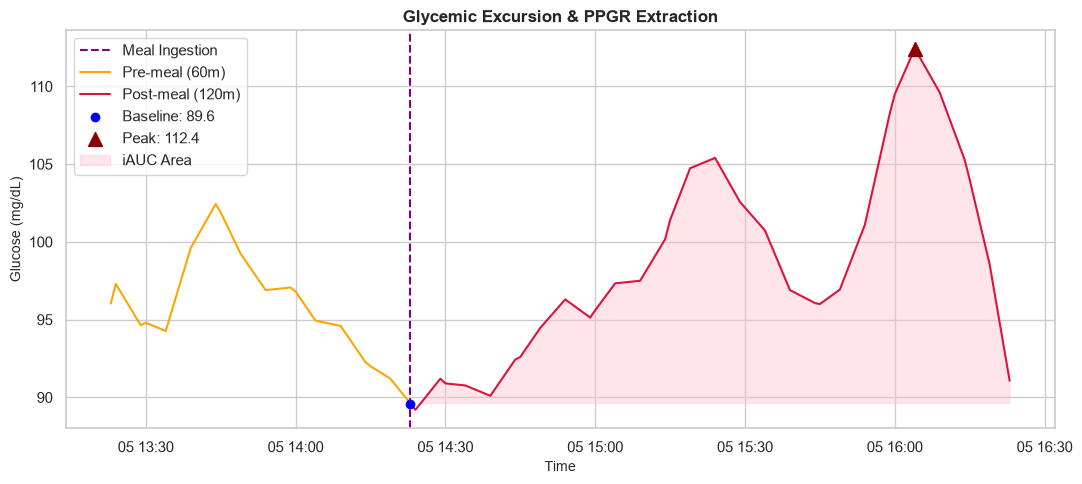
\includegraphics[width=0.9\columnwidth]{images/glycemic_excursion_and_ppgr_extraction.png}
\caption{Continuous meal windowing protocol: Extraction of the 60-minute pre-meal sequence ($\mathbf{X}_{\text{seq}} \in \mathbb{R}^{60 \times 3}$) and the 120-minute postprandial excursion target ($\mathbf{Y}_{\text{traj}} \in \mathbb{R}^{24}$).}
\label{fig:ppgr_extraction}
\end{figure}

\section{Summary of Static Feature Dimensionality}
Alongside the 60-minute dynamic inputs $\mathbf{X}_{\text{seq}}$, each meal sample includes a 61-dimensional static feature vector $\mathbf{x}_{\text{stat}} \in \mathbb{R}^{61}$ covering patient traits and nutritional values:
\begin{itemize}
    \item \textbf{Dietary Nutrients (7 features):} Net carbohydrates, dietary fiber, sugar, fat, protein, total calories, and the ratio of carbs to fiber.
    \item \textbf{Body Measurements (4 features):} Age, gender (one-hot encoded), body mass index (BMI), and weight in kilograms.
    \item \textbf{Clinical Blood Panel (20 features):} Fasting glucose, fasting insulin, HOMA-IR, HbA1c, lipid profiles (cholesterol, HDL, LDL, triglycerides), and complete blood count numbers.
    \item \textbf{Gut Functional Scores (22 features):} Biological pathway scores, including butyrate synthesis and LPS production capacity.
    \item \textbf{Microbiome Representation Latents (8):} The 8-dimensional continuous latent vector ($\mathbf{z}_{\text{microbiome}} \in \mathbb{R}^8$) derived via our deep $\beta$-Variational Autoencoder (detailed in Chapter \ref{chap:microbiome_vae}).
\end{itemize}
